\documentclass[a4paper, 8pt]{article}

%spacing
\usepackage[compact]{titlesec}
\titlespacing{\section}{0pt}{*1}{*1}
\titlespacing{\subsection}{0pt}{*1}{*1}
\raggedbottom

%science unit
\usepackage{siunitx}

%image insertion
\usepackage{graphicx} %image settings
\DeclareGraphicsExtensions{.pdf,.png,.jpg, .gif}

%math
\usepackage{amsmath} %math
%\usepackage{cmbright} %math font

%font
\usepackage{kotex}
\usepackage{fontspec}
\ifx가가
\setmainhangulfont[Ligatures=TeX,
BoldFont={KoPubBatang Medium}]{KoPubBatang Light}
\setsanshangulfont[Ligatures=TeX,
BoldFont={KoPubDotum Medium}]{KoPubDotum Light}
\setmainhanjafont[Ligatures=TeX,
BoldFont={KoPubBatang Medium}]{KoPubBatang Light}
\setsanshanjafont[Ligatures=TeX,
BoldFont={KoPubDotum Medium}]{KoPubDotum Light}
\xetexkofontregime[puncts=prevfont, colons=prevfont, cjksymbols=hangul]{latin}
\fi

%줄간격
\usepackage{setspace}
\usepackage{indentfirst}
\setstretch{1.3}
\everydisplay{\setstretch{1.2}}

%subfigure
\usepackage{subfigure}

%ccaption
\usepackage{ccaption}
\newfixedcaption{\outfigcaption}{figure}
\newfixedcaption{\outtabcaption}{table}

%caption size
\usepackage[font={footnotesize}]{caption}

\pagestyle{plain}
\title{물리 실험보고서 2}
\author{이한빈, 의예과 2016-XXXXX}

\begin{document}


\numberwithin{equation}{section}
\maketitle

\section{Introduction}


	축전기는 전하를 저장하는 장치로 전압이 가해졌을 때 전압에 비례하는 양의 전하를 축적한다.
		\begin{equation} \label{eq:qcv}
			Q=CV
		\end{equation}

	(\ref{eq:qcv})에 쓰인 비례상수 C는 축전기의 기하학적 모양과 유전체의 종류에 의존한다. 본 실험에 쓰여진 평행판 축전기의 경우 극판의 면적이 $A$, 극판의 간격이 $d$일 때 다음으로 주어진다.
		\begin{equation} \label{eq:ppl}
			C=\epsilon \frac{A}{d} \quad (단, \: \epsilon는 \: 극판 \: 사이의  \: 유전상수)
		\end{equation}

	축전기의 모습을 그림으로 나타내면 다음과 같다.
		\begin{figure}[h]
			\centering
				\subfigure[Parallel Plate Capacitor]{
				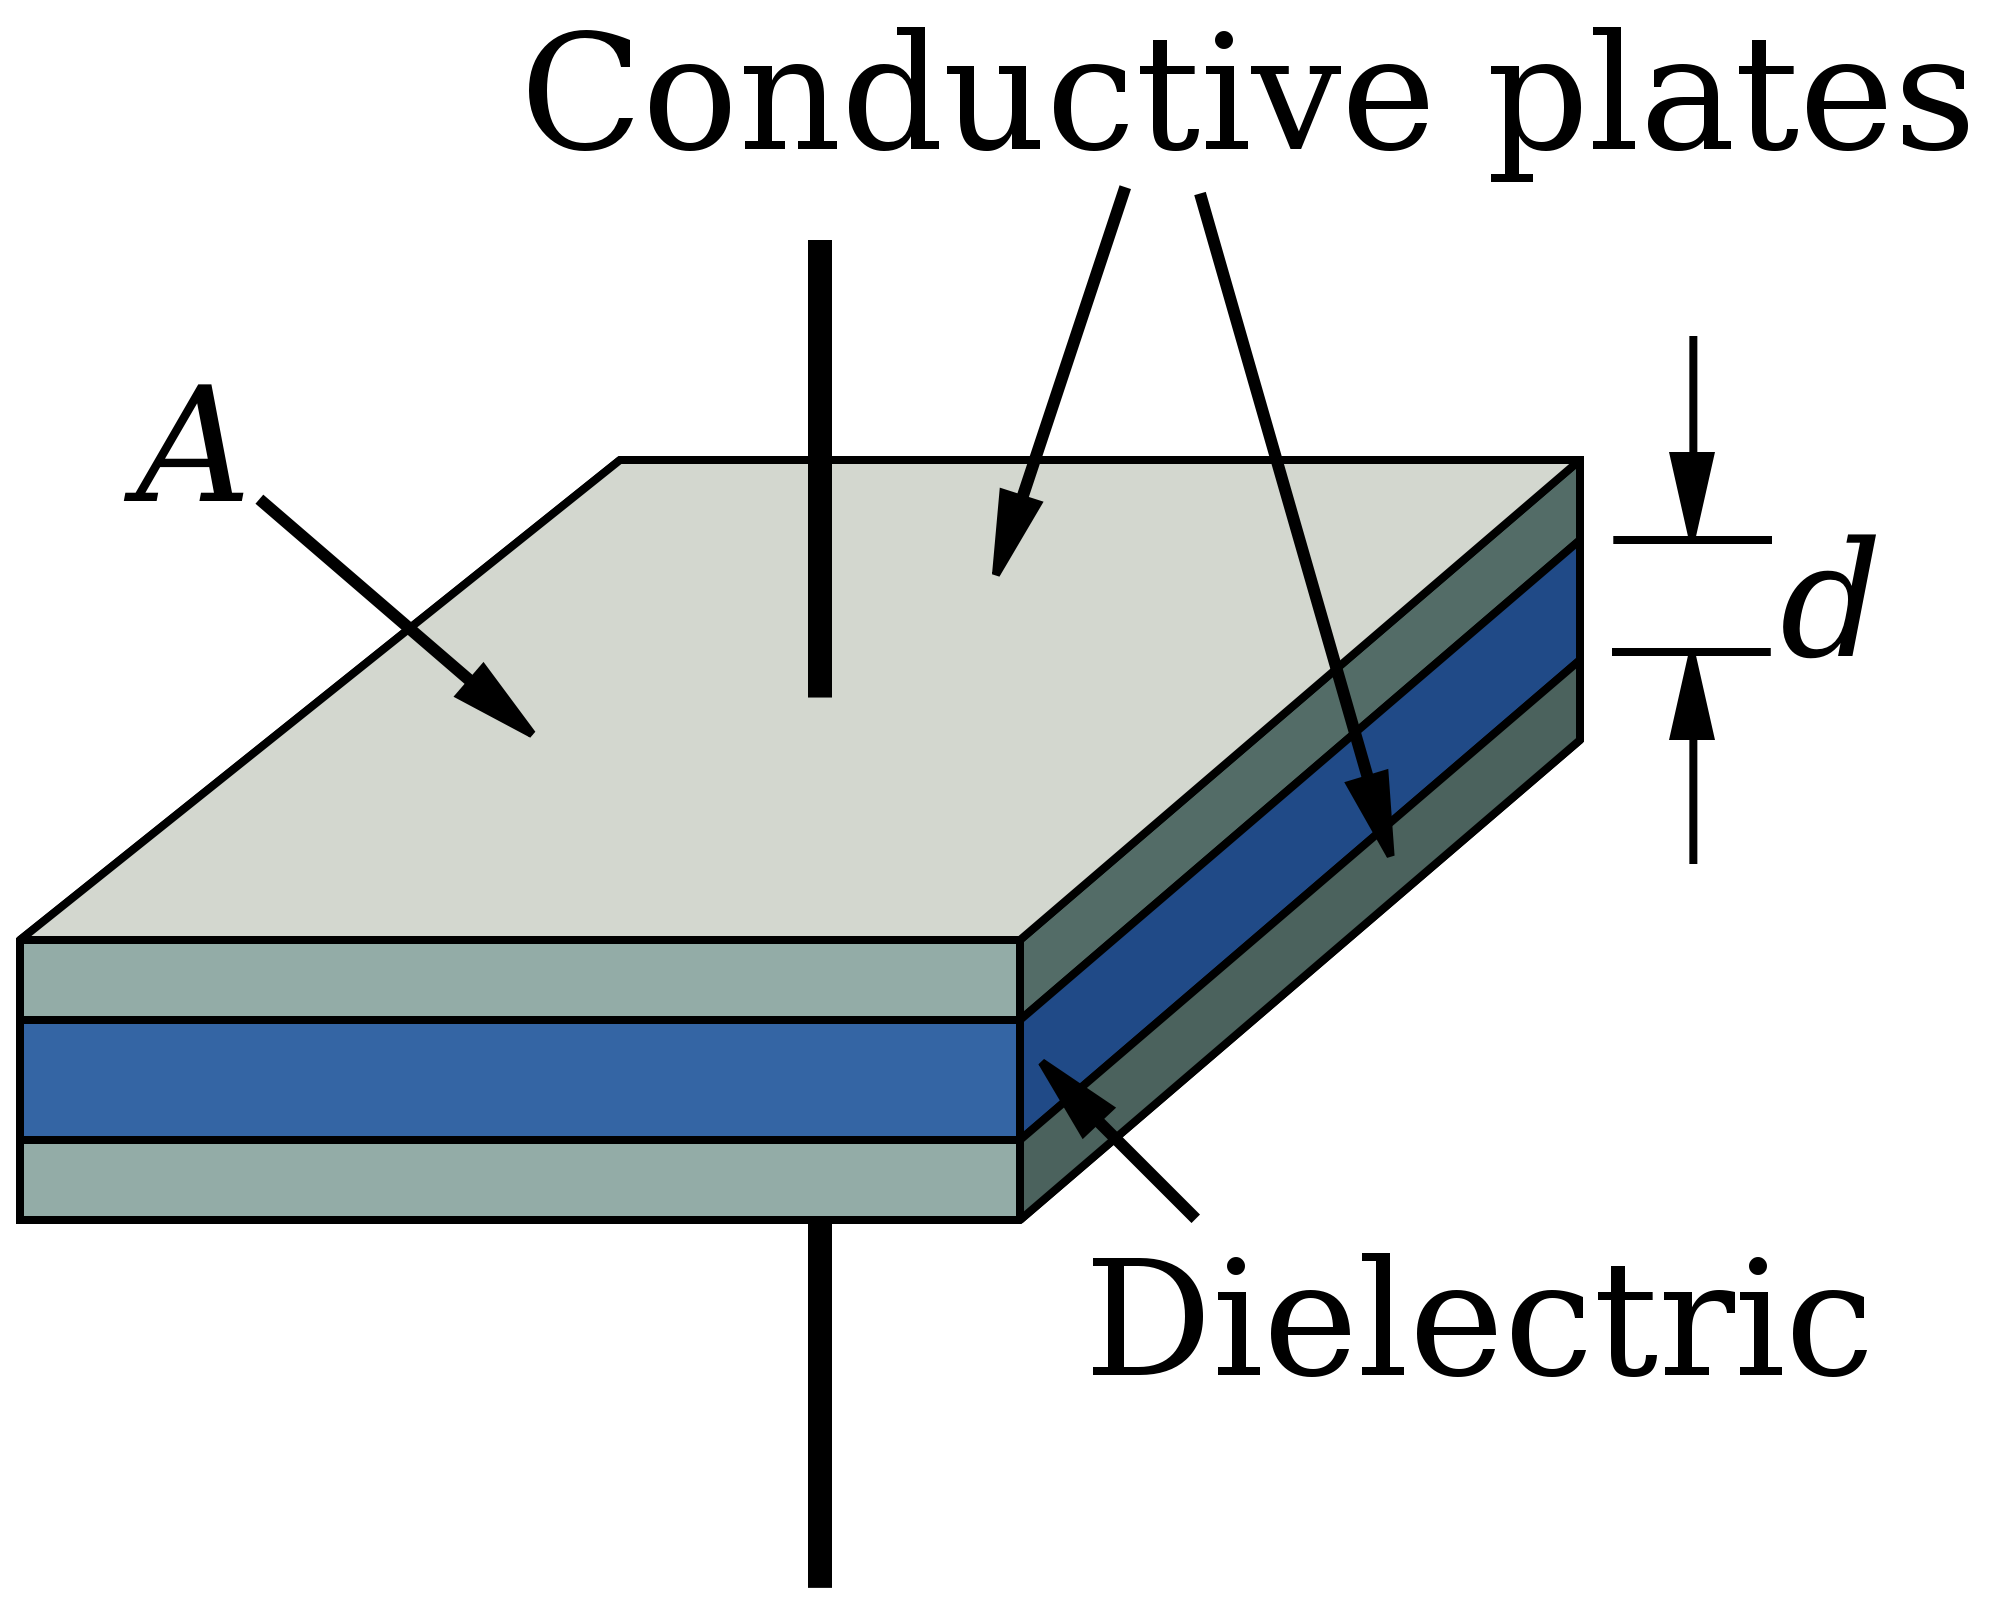
\includegraphics[width=0.4\textwidth]{img/plate1.png}
				\label{fig:plate1}	
				}
			\quad
				\subfigure[Edge Effect]{
				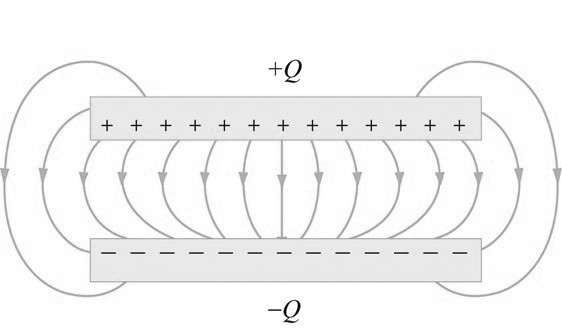
\includegraphics[width=0.4\textwidth]{img/edgeeff.jpg}
				\label{fig:edge}
				}
			\caption{Parallel Plate Capacitor and it's Edge Effect}
		\end{figure}
	
	무한히 넓은 이상적인 평행판 축전기의 전기력선은 평행하지만 유한한 크기의 평행판 축전기의 전기장은 Figure \ref{fig:edge}
	처럼 모서리에 가까워질수록 휘어진다. 이를 Edge Effect라고 한다. 그러나 A가 d에 비혜 충분히 크면 Edge Effect는 무시할 수 있을만큼 작아지므로 본 실험에서는 축전기의 전기장이 평행하다고 가정한다. 

\newpage
	본 실험에서는 전압과 축전기의 기하학적 구조를 바꿨을 때 축전기 극판 사이의 힘이 어떻게 변하는지 살펴보았다. 축전기에 걸린 전압을 $V$, 축전기의 간격을 $d$라고 했을 때 축전기의 사이의 전기장은 다음과 같다.
		\begin{equation} \label{eq:efd}
			E=\frac{V}{d}
		\end{equation}
	그런데 이 전기장은 두 극판이 만들어낸 전기장의 합이므로 한 쪽 극판이 받는 전기장은 (\ref{eq:efd})의 절반인 $E=V/{2d}$이다.

	극판이 받는 힘은 $F=QE$이고 $Q=CV$이므로 식(\ref{eq:ppl})을 대입하면 다음을 얻는다. 
		\begin{equation} \label{eq:force}
			F=\frac{\epsilon{}AV^{2}}{2d^{2}}
		\end{equation}


	축전기는 회로 요소이므로 병렬연결, 직렬연결에 대한 합성 전기용량을 구할 수 있다.
	축전기가 병렬연결되어있을 경우 양 극판에 걸린 전압의 크기가 $V$로 같고 총 전하량은 $Q=Q_1+Q_2$이므로 식(\ref{eq:qcv})을 대입하면 다음을 얻는다. 
		\begin{equation}
			CV=Q=Q_{1}+Q_{2}=C_{1}V+C_{2}V=(C_{1}+C_{2})V 
		\end{equation}

	이를 정리하면 다음과 같다.
		\begin{equation}
			C=C_{1}+C_{2}
		\end{equation}
	
	축전기가 직렬연결되어있을 경우 두 극판에 축적된 전하의 크기가 같고 총 전압은 $V=V_1+V_2$이므로 식(\ref{eq:qcv})을 대입하면 다음을 얻는다.
		\begin{equation}
			\frac{Q}{C}=V=V_{1}+V_{2}=\frac{Q}{C_1}+\frac{Q}{C_2}
		\end{equation}

	이를 정리하면 다음과 같다.
		\begin{equation}
			\frac{1}{C}=\frac{1}{C_1}+\frac{1}{C_2}
		\end{equation} 


	본 실험에서는 위의 식들을 이용하여 조건이 바뀌었을 때 두 극판 사이의 힘이 어떤 식으로 작용하는 지 알아본다. 

\newpage
\section{Method}
	\begin{figure}[h]
		\centering
		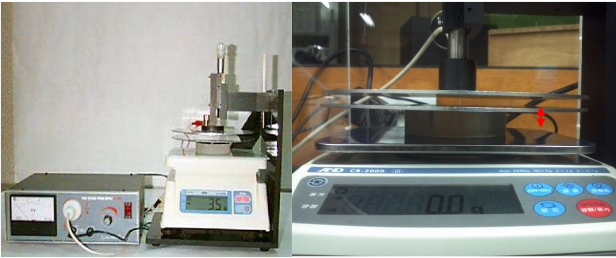
\includegraphics[width=0.7\textwidth]{img/expconfig.png}
		\caption{실험 장치}
	\end{figure}
	\noindent준비물: 전원, 저울, 전압계, 평행판 축전기, 평행판 거리 조절기, 1.35cm 유리판, 1.35cm 아크릴판\\
	\indent극판이 받는 힘이 바뀌면 극판이 저울에 가하는 수직항력이 바뀌므로 저울 값의 변화로부터 극판이 받는 힘의 변화를 측정할 수 있다. 따라서 거리 조절기로 극판 사이의 거리, 전원의 전압, 유전체의 유전율을 조절하면서 저울의 값을 기록하면 극판이 받는 힘의 변화와 앞선 물리량의 관계에 대해 알 수 있다.\\
	평행판의 반지름은 10\si{cm}으로 측정되었다.

\subsection{거리에 따른 전기력의 변화}
	전원의 전압을 5\si{kV}로 놓고 두 극판 사이에는 아무 것도 넣지 않았다($\epsilon{}_{air} \approx 1$).
	이 때 극판 사이의 거리 $d$를 각각 1.3, 1.2, 1.1, 1.0, 0.9, 0.8, 0.7\si{cm}로 놓고 전원 장치를 킨 후 저울에 나타난 숫자를 측정하였다.

\subsection{전압에 따른 전기력의 변화}
	극판 거리를 1\si{cm}로 놓고 두 극판 사이에는 아무 것도 넣지 않았다($\epsilon{}_{air} \approx 1$).
	이 때 전원의 전압 $V$를 각각 0, 1.5, 3, 4.5, 6, 7,5, 9\si{kV}로 놓고 전원 장치를 킨 후 저울에 나타난 숫자를 측정하였다. 
	전압의 간격을 1.5\si{kV}로 설정한 것은 1.5\si{kV}가 저울의 눈금변화가 나타난 최소 전압이었기 때문이다.

\subsection{유전율에 따른 전기력의 변화}
	극판 사이에 1.35\si{cm} 유리와 아크릴을 끼워넣었다. 1.35\si{cm}는 유리와 아크릴을 넣고 조였을 때의 간격이다.
	전압을 유리에서는 1\si{kV}, 아크릴에서는 2.5, 5\si{kV}로 설정했다. 
	유리에서는 1\si{kV}이상에서 장비에서 고주파음이 들려서 고주파음이 들리지 않는 최대치로 설정한 것이다. 
	그 이하에서는 저울의 눈금변화가 없어서 실험하지 못했다. 
	아크릴에서도 고주파음이 들리지 않는 최대치와 그 절반값을 실험대상으로 삼았다.  

\newpage

\section{Result}
	\subsection{거리에 따른 전기력의 변화}
	\vspace{-6.5mm}
	\begin{figure}[h]
		\centering
		\begin{minipage}{.27\textwidth}
			\centering
			\begin{tabular}{rrrrrrrr}
			\hline \hline
			$d$(\si{cm}) & $\Delta${}W(\si{g}) \\
			\hline
			1.3 & 1.0 \\
			\hline
			1.2 & 1.2 \\
			\hline
			1.1 & 1.4 \\
			\hline
			1.0 & 1.7 \\
			\hline
			0.9 & 2.0 \\
			\hline
			0.8 & 2.6 \\
			\hline
			0.7 & 3.4 \\
			\hline \hline
			\end{tabular}
		\end{minipage}
		\begin{minipage}{.7\textwidth}
			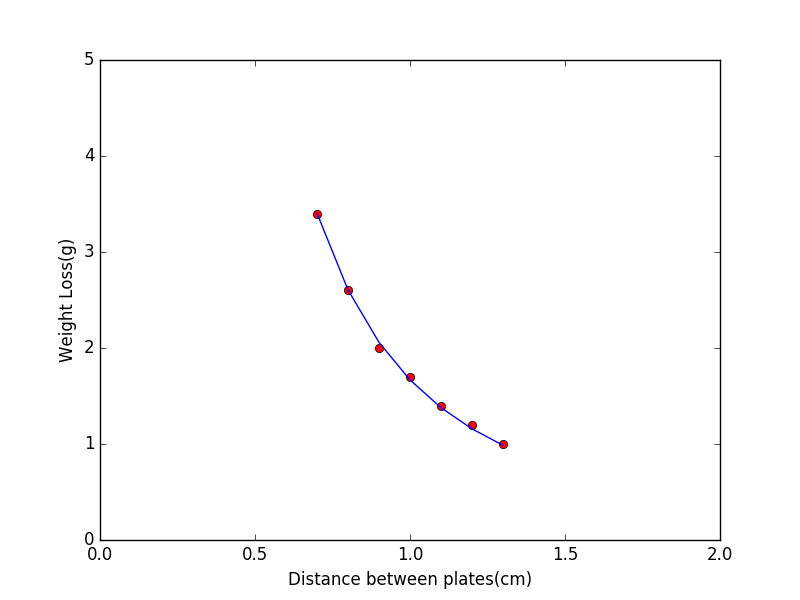
\includegraphics[width=\textwidth]{img/figure_1.png}
		\end{minipage}
		\caption{Relation between $d$(\si{cm}) and Weight Loss($\Delta$W)}
	\end{figure}
	Scipy에서 $y=a_{1}/{x^2}$로 Fitting한 결과 $a_{1}=1.64*10^{-6}\si{N\cdot{}m^{2}}$, $R^2=0.931$로 계산됐다.

	\subsection{전압에 따른 전기력의 변화}
	\vspace{-6.5mm}
	\begin{figure}[h]
		\centering
		\begin{minipage}{.27\textwidth}
			\centering
			\begin{tabular}{rrrrrrrr}
			\hline \hline
			$V$(\si{kV}) & $\Delta${}W(\si{g}) \\
			\hline
			0.0 & 0.0 \\
			\hline
			1.5 & 0.1 \\
			\hline
			3.0 & 0.6 \\
			\hline
			4.5 & 1.3 \\
			\hline
			6.0 & 2.4 \\
			\hline
			7.5 & 3.9 \\
			\hline
			9.0 & 5.6 \\
			\hline \hline
			\end{tabular}
		\end{minipage}
		\hspace{0.1cm}
		\begin{minipage}{.7\textwidth}
			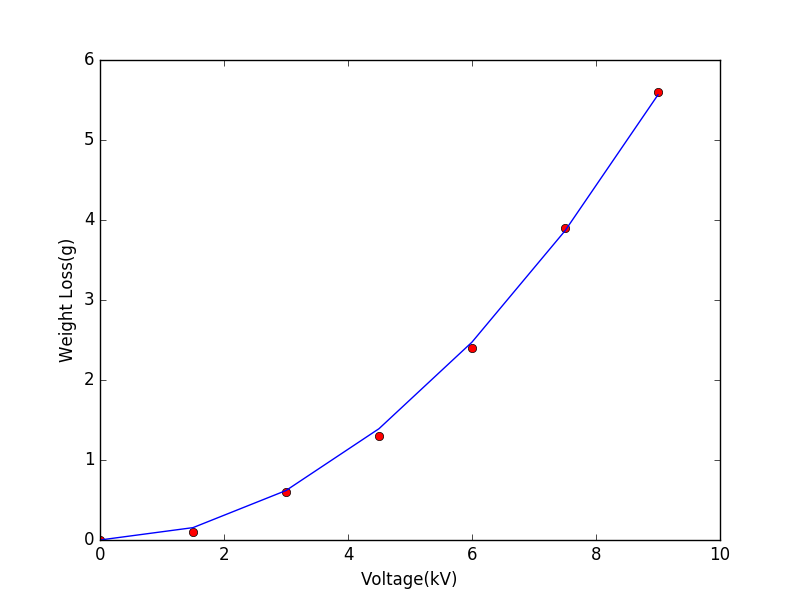
\includegraphics[width=\textwidth]{img/figure_2.png}
		\end{minipage}
		\caption{Relation between $V$(\si{kV}) and Weight Loss($\Delta$W)}
	\end{figure}
	Scipy에서 $y=a_{2}x^2$로 Fitting한 결과 $a_{2}=6.792*10^{-10}\si{N/V^{2}}$, $R^2=0.923$로 계산됐다.

	\subsection{유전율에 따른 전기력의 변화}
	유리($V=1\si{kV}$, $d=1.35{cm}$)와 아크릴($V=2.5, 5\si{kV}$, $d=1.35\si{cm}$)를 넣었을 때 무게 감소는 $25.6\si{g}$, $18.2\si{g}$, $28\si{g}$으로 측정됐다.

\newpage

\section{Conclusion}
	식 (\ref{eq:force})로부터 실험 1과 실험 2의 그래프가 각각 역제곱, 제곱에 비례하는 꼴일 것으로 예상하고 Fitting을 했다.
	그 결과 두 실험 모두 $R^2\ge0.9$로 이론과 실험이 잘 일치하는 것으로 나타났다.
	측정된 축전기의 값을 식 (\ref{eq:force})에 넣고 계산하면 
	$a_1=\epsilon{}_0AV^{2}/2=3.4\times10^{-6}$, $a_2=\epsilon{}_0A/2d^2=1.39\times10^{-9}$인데 이는 각각 2.1배, 2배 큰 값이다. 첫 번째 오차 원인은 축전기가 평행하지 않은 것 때문이었다. 
	유전체를 삽입한 이후 실험에서 유전체의 일부분은 강하게 조여졌지만 어떤 부분은 조여지지 않았던 것을 관찰했다. 따라서 $d$가 정확하게 측정되지 않은 것과 평행판으로 가정하고 계산된 식 (\ref{eq:force})이 실제와 다른 것이 오차의 원인이 된 것으로 보인다.

	유리의 경우 유전율이 $\epsilon{}_{glass}=2d^2F/AV^2=2.91\times10^{-9}\si{F/m}$로 계산되었는데 이는 실제 유전율인 $4.96\times10^{-11}\si{F/m}$보다 58배 크게 나타났다. 
	아크릴의 경우도 같은 계산을 통해 $\epsilon{}_{arc}=3.31\times10^{-10}\si{F/m}$으로 실제 값보다 14.6배 크게 나타났다. 
	두 번째 실험을 통해 얻은 값도 5.6배 크게 나타났다.
	실험에서는 크게 두 가지 오차 원인을 관찰할 수 있었다.
	먼저, 실험 3.1 및 3.2와 마찬가지의 이유로 d가 정확하게 측정되지 않았다.
	두 번째, $d$를 조절하는 장치가 저울에 추가적인 힘을 가했는데 이 값이 계속 변했다.
	영점을 조절하고 전압을 일정하게 맞춘 후에도 저울의 값이 계속 변하는 것을 관찰 가능했기 떄문이다.
	저울값의 변화가 없어진 후에 실험을 진행했지만 반복된 실험에서 그 설정값이 재현되지 않았기 때문에 신뢰할 수 없는 값이라고 볼 수 있다.
	추가적인 검증이 필요한 이유로는 레퍼런스에 기재된 유전체의 성분과 본 실험에서 사용한 유전체의 성분이 다르다는 것을 들 수 있다.  




	 
	
\section{Reference}
	1. Halliday, D., Resnick, R., \& Walker, J. (2014). {\it{}Principles of Physics} (10th ed., Vol. 2). Hoboken, NJ: Wiley. 
\end{document} 

%실험에서 개선할 점 등 피피티에서 봤던 거 모두 적어서 처리합시다.
